\documentclass{beamer}


% For TikZ flowchart
%\usepackage{tikz}
%\usetikzlibrary{shapes.geometric, arrows}
%\tikzstyle{startstop} = [rectangle, rounded corners, minimum width=3cm, minimum height=1cm,text centered, draw=black, fill=red!30]
%\tikzstyle{io} = [trapezium, trapezium left angle=70, trapezium right angle=110, minimum width=3cm, minimum height=1cm, text centered, draw=black, fill=blue!30]
%\tikzstyle{process} = [rectangle, minimum width=3cm, minimum height=1cm, text centered, draw=black, fill=orange!30]
%\tikzstyle{decision} = [diamond, minimum width=3cm, minimum height=1cm, text centered, draw=black, fill=green!30]
%\tikzstyle{arrow} = [thick,->,>=stealth]


\mode<presentation>
{
  \usetheme{Hannover}      % or try Darmstadt, Madrid, Warsaw, ...
  \usecolortheme{orchid} % or try albatross, beaver, crane, ...
  \usefonttheme{default}  % or try serif, structurebold, ...
  \setbeamertemplate{navigation symbols}{}
  \setbeamertemplate{caption}[numbered]
} 


\usepackage[printwatermark]{xwatermark}
\usepackage{xcolor}
\usepackage{graphicx}
\usepackage{lipsum}
%\usepackage{epsdice} %for dice symbols
%\usepackage{bbding} %for check boxes


\title{A Genetic Algorithm Approach to Finding an Optimal Strategy for a Folk Dice Game}
\date{January 3, 2017}
\author{David Ebert}
\institute{Tarleton State University}

\begin{document}
\maketitle

\section{Rules}
  \begin{frame}{How to Play Fargo}
  A player begins her turn by rolling 10 dice. Dice are scored as follows:
  \begin{enumerate}
  \item Three of a kind $n$ is worth $100n$ points, except three 1's count as 1000 points.
  %\item After triples are removed, \epsdice{1}'s are worth 100 points each.
  %\item After triples are removed, \epsdice{5}'s are worth 50 points each.
  \end{enumerate}
  \vspace{15 pt}
  %Upon scoring the dice and removing all triples, \epsdice{1}'s, and \epsdice{5}'s, a player may keep the points in her run and end her turn or continue rolling the scoring dice, thereby adding to the run's score. 
  \end{frame}

  \begin{frame}{How to Play Fargo}
  If a run is continued indefinitely, it will end in one of two ways:
  \begin{enumerate}
  \item If 0 points are added to a run's score after a re-roll, then the entire run is worth 0 and the turn is ended.
  \item If a run ends by running out of dice, then the run's score is added to that player's score and the player begins a new run of 10 dice.
  \end{enumerate}
  \end{frame}

  \begin{frame}{Example Turn}
  \centering
  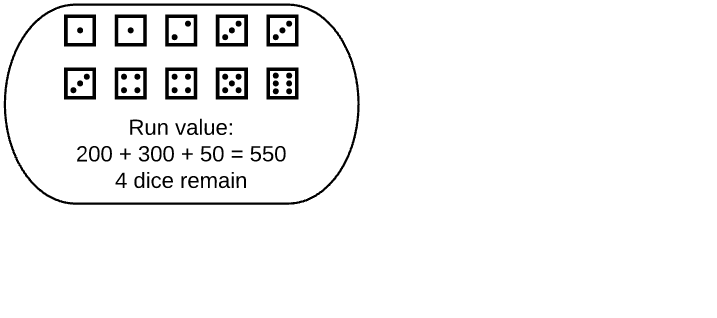
\includegraphics[width = \textwidth]{turn1_1.png}
  \end{frame}

  \begin{frame}{Example Turn}
  \centering
  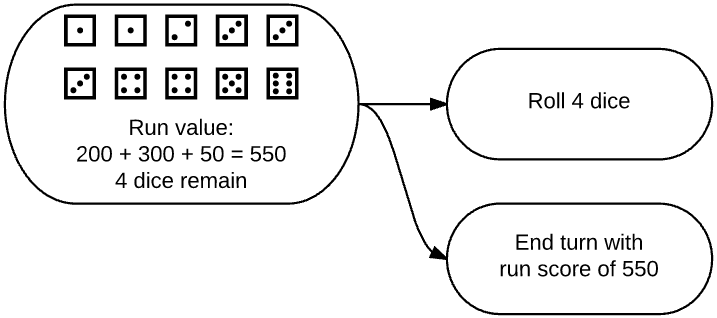
\includegraphics[width = \textwidth]{turn1_2.png}
  \end{frame}

  \begin{frame}{Example Turn}
  \centering
  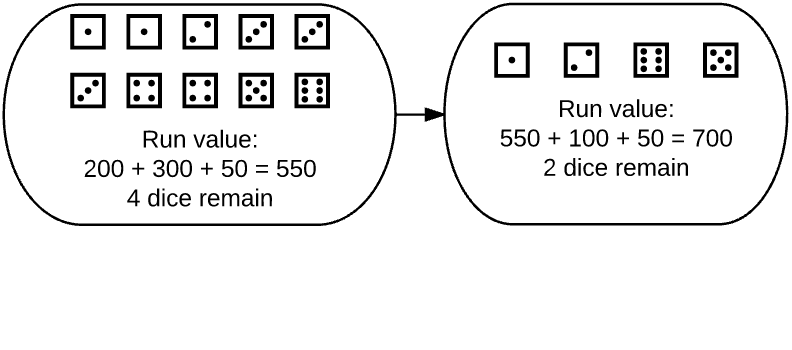
\includegraphics[width = \textwidth]{turn1_3.png}
  \end{frame}

  \begin{frame}{Example Turn}
  \centering
  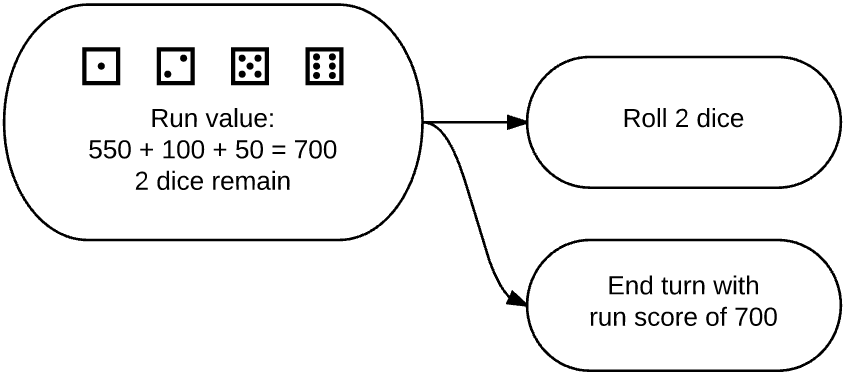
\includegraphics[width = \textwidth]{turn1_4.png}
  \end{frame}

  \begin{frame}{Example Turn}
  \centering
  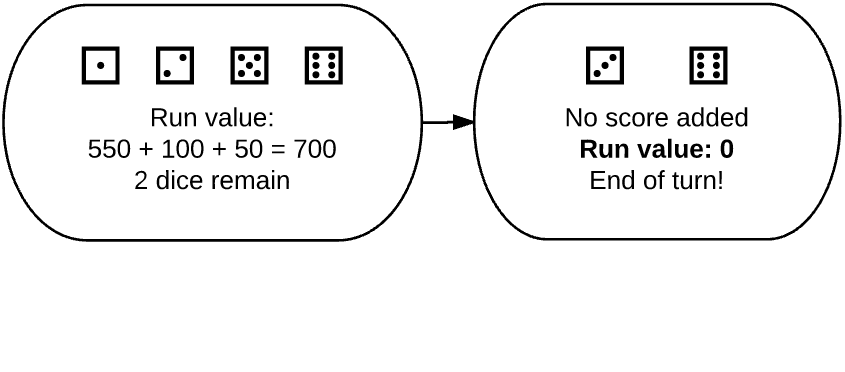
\includegraphics[width = \textwidth]{turn1_5.png}
  \end{frame}

  \begin{frame}{How (not) to Play Fargo}
  \textbf{Endgame}: 
  After a player ends his or her turn with 10,000 or more points, all other players may take one more turn, then the player with the highest score wins.
  
  \begin{table}
  \centering
  \begin{tabular}{|c|c|}
  \hline
  \multicolumn{2}{|c|}{\textbf{Final Scores}} \\ \hline
Adam                  & 10,750              \\ \hline
Mary                  &  8,300              \\ \hline
Mikaela               &  9,250              \\ \hline
Parker                &  1,750              \\ \hline
Steph                 &  6,100              \\ \hline
\textbf{Me}           & \textbf{0}          \\ \hline
  \end{tabular}
  \end{table}
  \end{frame}

%  \begin{frame}{Similar Dice Games}
%  \begin{itemize}
%      \item Yahtzee: Solved using Markov chains.
%      \item Farkle: Similar repeated runs and risk of losing everything, but more complicated decision tree.
%  \end{itemize}
%  \end{frame}








\section{Strategy Space}
  \begin{frame}{Questions}
  \begin{itemize}
  	\item[$\square$] How many strategies are there?
    \item[$\square$] What's the expected value of a strategy?
    \item[$\square$] Which strategy is the best?
  \end{itemize}
  \end{frame}

  \begin{frame}{Strategy Space}
  Two Observations:
  	\begin{itemize}
    \item If a reasonable strategy continues rolling $n$ dice and $p$ points, then it should also continue rolling with $n$ dice and $<p$ points. 
    \item A player should always roll 9 or 10 dice, since it's impossible to lose.
    \end{itemize}
  \end{frame}

  \begin{frame}{Strategy Space}
	\begin{table}[]
	\centering
	\begin{tabular}{|c|c|c|}
	\hline
Dice      & Minimum    & Maximum   \\
Remaining & Score      & Score     \\ 
          & Possible   & Possible  \\ \hline
1         & 450        & 3000      \\ \hline
2         & 400        & 2200      \\ \hline
3         & 350        & 2100      \\ \hline
4         & 300        & 2000      \\ \hline
5         & 250        & 1200      \\ \hline
6         & 200        & 1100      \\ \hline
7         & 150        & 1000      \\ \hline
8         & 100        & 200       \\ \hline
	\end{tabular}
  \end{table}
  \end{frame}

  \begin{frame}{Strategy Space}
  \textbf{Conclusion}: All reasonable Fargo strategies can be written as a list of $x_1, x_2, ..., x_8$, where $x_i$ indicates that with $i$ dice remaining a player should continue rolling unless their score is at least $x_i$.
  \end{frame}
  
  \begin{frame}{Strategy Space}
  \textbf{Example}: \\
  Consider the strategy vector \\
  \smallskip
  \begin{center}
  [450, 600, 700, 650, 500, 1000, 1000, 250] \\
  \end{center}

  \medskip
  \hspace{5 pt} With one die, always stop rolling \\
  \hspace{5 pt} With 2 dice, keep rolling unless the run is worth at least 600 \\
  \hspace{5 pt} With 3 dice, keep rolling unless the run is worth at least 700 \\
  \hspace{100 pt}  \vdots \\
  \hspace{5 pt} With 7 dice, keep rolling unless the run is worth at least 1000 \\
  \hspace{5 pt} With 8 dice, always keep rolling
  \end{frame}
  
  \begin{frame}{Strategy Space}
\begin{table}[]
\centering
\begin{tabular}{|c|c|c|c|}
\hline
$i$ & min$(x_{i})$ & max$(x_{i})$ & count$(x_{i})$ \\ \hline
1 & 450       & 3050      & 52           \\ \hline
2 & 400       & 2250      & 37           \\ \hline
3 & 350       & 2150      & 36           \\ \hline
4 & 300       & 2050      & 35           \\ \hline
5 & 250       & 1250      & 20           \\ \hline
6 & 200       & 1150      & 19           \\ \hline
7 & 150       & 1050      & 18           \\ \hline
8 & 100       & 250       & 4            \\ \hline
\end{tabular}
\end{table}

Total number of \textit{reasonable} strategy vectors: 
$$\prod_{i=1}^{8} \text{count}(x_{i} s) = 66 327 206 400 > 66 \text{ billion}$$
  \end{frame}





\section{Expected Value}
  \begin{frame}{Questions}
  \begin{itemize}
  	%\item[\Checkmark] How many strategies are there?
    \item[$\square$] What's the expected value of a strategy?
    \item[$\square$] Which strategy is the best?
  \end{itemize}
  \end{frame}

%  \begin{frame}{Expected Value}
%\begin{table}[]
%\centering
%\begin{tabular}{|c|c|c|}
%\hline
%$i$  & Ways to roll $i$ dice & Scoring outcomes rolling $i$ dice \\ \hline
%1  & 6                        & 3                                 \\ \hline
%2  & 21                       & 6                                 \\ \hline
%3  & 56                       & 13                                \\ \hline
%4  & 126                      & 25                                \\ \hline
%5  & 252                      & 39                                \\ \hline
%6  & 462                      & 59                                \\ \hline
%7  & 792                      & 87                                \\ \hline
%8  & 1287                     & 117                               \\ \hline
%9  & n/a                      & n/a                               \\ \hline
%10 & 3003                     & 194                               \\ \hline
%\end{tabular}
%\end{table}
%  \end{frame}

  \begin{frame}{Expected Value}
    \centering
    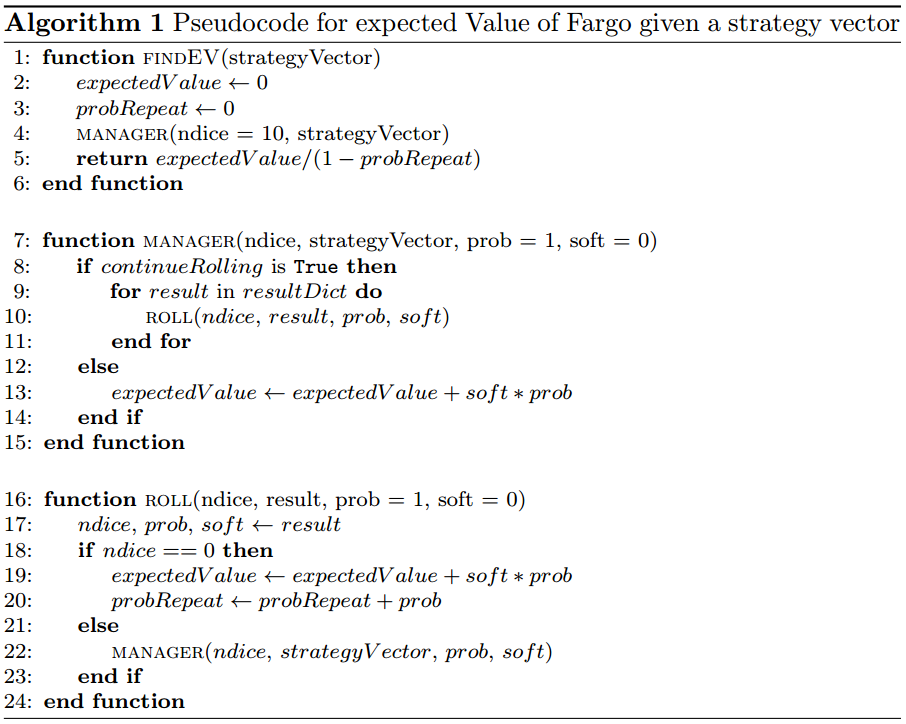
\includegraphics[width = 0.8\textwidth]{pseudocode.png}
  \end{frame}

  \begin{frame}{Expected Value}
  	\begin{align*}
\text{EV}(\text{Turn}|\text{Strategy}) &= 
\Sigma \text{Outcome Score} \times \text{P}(\text{Outcome}) \\
&+  \text{EV}(\text{Turn}|\text{Strategy})\times \text{P}(\text{Repeated Run}) \\
\\
\\
\text{EV}(\text{Turn}|\text{Strategy}) &= 
\frac{\Sigma \text{Outcome Score} \times \text{P}(\text{Outcome})}{1-\text{P}(\text{Repeated Run})}
    \end{align*}

\vspace{15 pt}

  Using a recursive function, it is easy to find a strategy vector's expected value.
  \end{frame}










\section{Genetic Algorithm}
  \begin{frame}{Questions}
  \begin{itemize}
  	%\item[\Checkmark] How many strategies are there?
    %\item[\Checkmark] What's the expected value of a strategy?
    %\item[$\square$] Which strategy is the best?
  	\item How many strategies are there?
    \item What's the expected value of a strategy?
    \item Which strategy is the best?
  \end{itemize}
  \end{frame}
  
  \begin{frame}{Genetic Algorithm}
  \begin{itemize}
  \item Introduced by John Holland in the 1970's to explore large solution spaces by mimicking the process of natural selection.
  \item Applications include the vehicle routing problem, 3D simulated muscles, wind turbine placement, machine learning, \& spacecraft antennae.
  \end{itemize}
  \end{frame}

  \begin{frame}{Genetic Algorithm}
	3 ingredients:
	\begin{enumerate}
		\item Problem encoding (strategy vectors)
		\item Evaluation function (expected value)
		\item Rules for genetic succession
	\end{enumerate}
  \end{frame}

  \begin{frame}{Genetic Algorithm}
  Generation 1: \\
  	\hspace{18 pt} Select 1000 random strategy vectors (starting population) \\
  \medskip
   Generation 2:
    \begin{enumerate}
    \item Sort 1000 strategies from generation 1 by EV
    \item Keep the best 250 strategies (survival of fittest)
    \item Add 20 random strategies (2\% genetic diversity) 
    \item Randomly combine strategies until there are 1000 strategies (genetic recombination)
    \item Randomly change 10 entries (1\% mutation)
  \end{enumerate}
  \end{frame}

  \begin{frame}{Genetic Algorithm}
  Generation 1: \\
  	\hspace{18 pt} Select 1000 random strategy vectors (starting population) \\
  \medskip
   Generation $n>1$:
    \begin{enumerate}
    \item Sort 1000 strategies from generation $n-1$ by EV
    \item Keep the best 250 strategies (survival of fittest)
    \item Add 20 random strategies (2\% genetic diversity) 
    \item Randomly combine strategies until there are 1000 strategies (genetic recombination)
    \item Randomly change 10 entries (1\% mutation)
  \end{enumerate}
  \end{frame}
  
  \begin{frame}{Results}
  \begin{center}
  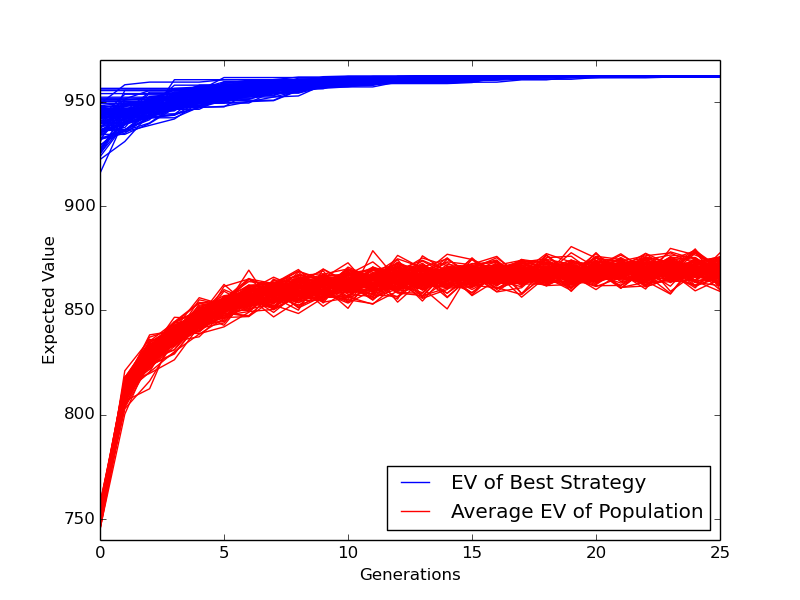
\includegraphics[width = 0.8\textwidth]{100trials.png}
  \end{center}

    Results from 100 trials with a population of 1000 strategies over 25 generations.
  \end{frame}

  \begin{frame}{Results}
  \begin{center}
  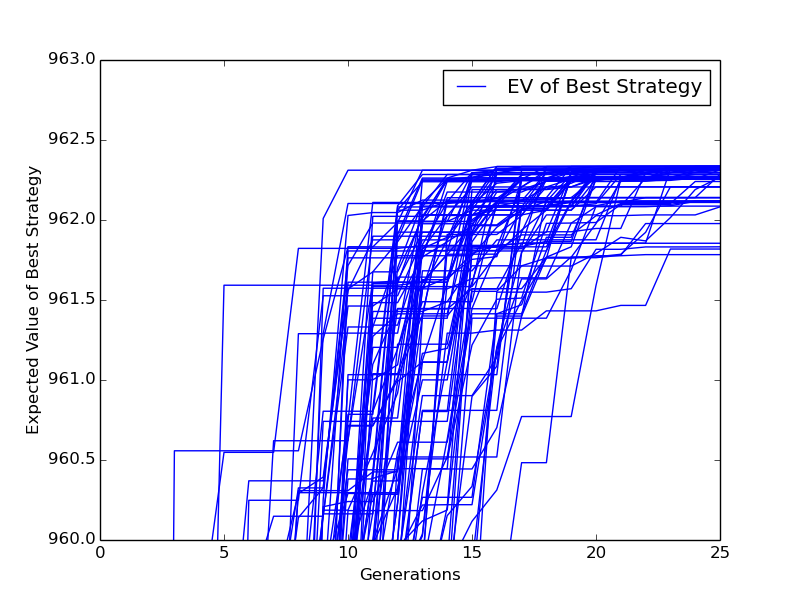
\includegraphics[width = 0.8\textwidth]{100trials2.png}
  \end{center}
  
    Results from 100 trials with a population of 1000 strategies over 25 generations.
  \end{frame}

  \begin{frame}{Results}
  \begin{itemize}
  	\item Maximum EV of 962.3343332342337 attained by 8/100 trials with the following strategy vector: \\
    \begin{center}
    [550, 400, 550, 1150, 1250, 1150, 1050, 250]
    \end{center}
    \item Among the highest-EV vectors from each trial, the mean vector is 2.42 \textit{steps} away from the best strategy, and the farthest vector was 7 \textit{steps} away.
  \end{itemize}
  \end{frame}


  \begin{frame}{Results}
	\textbf{Aggressiveness}: 
    
    For each strategy vector $x_1, ..., x_8$, define the \textit{aggressiveness} of the vector as $a_1, ..., a_8$, where each $a_i$ denotes the fraction of possible values for $x_i$ that are smaller than $x_i$.
  \end{frame}
  
    \begin{frame}{Strategy Space}
	\begin{table}[]
	\centering
	\begin{tabular}{|c|c|c|c|c|c|c}
	\hline
$i$  & min($x_i$) & max($x_i$)  & & $x_i$ from Best Strategy & Aggressiveness $a_i$  \\ \hline
1    & 450        & 3050        & & 550           & 2$/$52  \\ \hline
2    & 400        & 2250        & & 400           & 0       \\ \hline
3    & 350        & 2150        & & 550           & 4$/$36  \\ \hline
4    & 300        & 2050        & & 1150          & 17$/$35 \\ \hline
5    & 250        & 1250        & & 1250          & 1       \\ \hline
6    & 200        & 1150        & & 1150          & 1       \\ \hline
7    & 150        & 1050        & & 1050          & 1       \\ \hline
8    & 100        & 250         & & 250           & 1       \\ \hline
	\end{tabular}
  \end{table}
    Aggressiveness of [550, 400, 550, 1150, 1250, 1150, 1050, 250] strategy vector, which yielded the highest EV of 962.3343332342337.
  \end{frame}

  \begin{frame}{Results}
  \begin{center}
  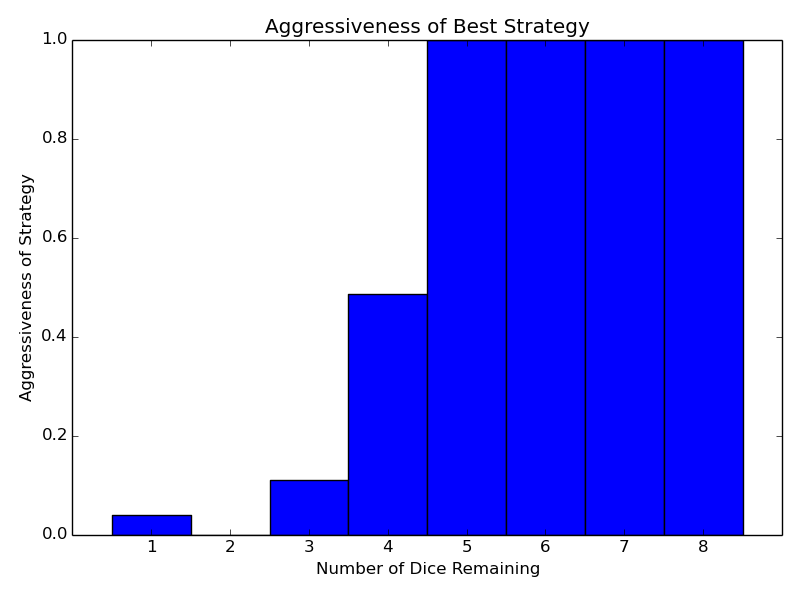
\includegraphics[width = 0.7\textwidth]{aggressiveness_barplot.png}
  \end{center}
  Aggressiveness of [550, 400, 550, 1150, 1250, 1150, 1050, 250] strategy vector, which yielded the highest EV of 962.3343332342337.
  \end{frame}







\section{Conclusions}
  \begin{frame}{Questions}
  \begin{itemize}
  	%\item[\Checkmark] How many strategies are there?
    %\item[\Checkmark] What's the expected value of a strategy?
    %\item[\Checkmark] Which strategy is (probably) the best? 
    \item How many strategies are there?
    \item What's the expected value of a strategy?
    \item Which strategy is (probably) the best? 
    
  \end{itemize}
  \end{frame}
  
  \begin{frame}{Conclusions and Future Work}
  \begin{itemize}
  \item The genetic algorithm efficiently and consistently yields a viable strategy.
  \item More work is necessary to confirm the optimal strategy and make the genetic algorithm more efficient.
  \item The genetic algorithm and EV algorithm are likely to extend to further analyses of Fargo, including the multi-player game and end-game strategies.
  \end{itemize}
  \end{frame}

  \begin{frame}{Questions?}
  \begin{itemize}
  \item Python code repository:  \url{https://github.com/dpebert7/fargo}
  \vspace{5 pt}
  \item \url{david.ebert@go.tarleton.edu}
  \vspace{5 pt}
  \item Special thanks to Dr. Jesse Crawford for his insight and inspiration
  
  \end{itemize}

  \end{frame}
\end{document}